\documentclass{../res/univ-projet}

%Import des packages utilisés pour le document
\usepackage[utf8x]{inputenc}
\usepackage[francais]{babel}
\usepackage[T1]{fontenc}
%\usepackage{array}
%\usepackage{hyperref}
%\usepackage{tabularx, longtable}
%\usepackage[table]{xcolor}
%\usepackage{fancyhdr}
%\usepackage{lastpage}
\usepackage{../res/tikz-uml}
\usepackage{tikz}
\usepackage{calc}
\usepackage{xstring}
\usepackage{pgfopts}

\definecolor{gris}{rgb}{0.95, 0.95, 0.95}

%Redéfinition des marges
%\addtolength{\hoffset}{-2cm}
%\addtolength{\textwidth}{4cm}
\addtolength{\topmargin}{-1cm}
\addtolength{\textheight}{1cm}
\addtolength{\headsep}{0.8cm} 
\addtolength{\footskip}{-0.2cm}


%Import page de garde et structures pour la gestion de projet
%\usepackage{structures}

%Variables
\logo{../res/logo_univ.png}
\title{Rapport de projet}
\author{Pierre \bsc{Balmelle},\\ Lucas \bsc{Barbay},\\ Bertille \bsc{Bouillie},\\ Matthieu \bsc{Fin},\\ Guillaume \bsc{Leroy},\\ Ibrahima \bsc{Sorry Barry},\\ Olivier \bsc{Thibault}}
\projet{Projet PGP}
\projdesc{Étude et implantation d'un outil graphique de gestion de clefs PGP}
\filiere{Master 1 SSI }
\matiere{Conduite de projet}
\date{\today}

% -- Début du document -- %
\begin{document}

%Page de garde
\maketitle
\newpage
%La table des matières
\tableofcontents

\newpage

\section{Introduction}

Nous allons vous présenter dans ce rapport une synthèse du projet "Etude et implantation d'un outil graphique de gestion de clef PGP". Ce document vous permettra de comprendre ce qui a été réalisé dans ce projet d'un point de vue fonctionnel mais aussi technique. Nous parlerons également de la gestion de projet qui nous a permis de réaliser ce projet.

  \subsection{Contexte}
   % Sujet
  % Equipe
  % Cadre 
  Ce projet a été réalisé dans le cadre de la première année du Master Sécurité des Système d'informations enseigné à  l'Université de Rouen. Ce projet est découpé en deux parties et a commencé au début de l'année. Il nous a été demandé au premier semestre de rédiger les documents de Gestion de projets qui ont servi de base durant toute la durée du projet. Au second semestre il a fallu développer l'application en s'aidant des documents rédigés et en les faisant évoluer au fur et à mesure du projet.
  \subsection{L'équipe}
  L'équipe de ce projet était composée au début de 7 étudiants en première année du master évoqué ci-dessus : Pierre Balmelle, Lucas Barbay, Bertille Bouillie, Mathieu Fin, Guillaume Leroy, Ibrahima Sorry Barry et Olivier Thibault. Nous avons du réaliser ce projet dans le cadre du module de gestion de projet sous la tutelle de Monsieur Karim ABDELLAH GODARD. et grâce aux cours de Monsieur Remi DIONISI. Le sujet de ce projet nous a été donné par Magalie Bardet, enseignante-chercheuse à l'Université de Rouen.

\section{Présentation du projet initial}

Pour introduire ce projet, nous allons commencer par parler du standard OpenPGP. Ce standard est un format de cryptographie normalisé dans la RFC 4880. OpenPGP décrit le format des messages qui sont adaptés aux outils permettent l'envoie sécurisés de message ou bien le stockage de message.
GnuPG (GNU Privacy Guard) est un de ces outils. Il se base sur le logiciel PGP et utilise un système hybride liant cryptographie symétrique et asymétrique pour permettre l'envoie de message chiffrés et/ou signés. Pour pouvoir s'échanger des messages, les utilisateurs de GPG doivent s'envoyer leur clé publique qui servira au chiffrement des messages.

  \subsection{Objectifs}
  L'objectif de ce projet est de développer un outil graphique de gestion de clefs PGP. Il existe déjà plusieurs éditeurs permettant d'utiliser GPG graphiquement mais aucun ne permettent une gestion fine des clefs et la partie toile de confiance n'est pas intuitive. Il nous est donc demandé de réaliser une interface qui soient plus complète que les outils existants. L'objectif est dans un premier temps d'étudier complètement GnuPG et OpenPGP pour comprendre parfaitement son utilisation et réaliser un logiciel le plus exhaustif possible. L'interface réalisée devra permettre aux utilisateurs de faire des réglages techniques qu'ils soient experts ou novices. Un document expliquant les fonctionnalités devra être livré avec le projet.
  Enfin il est demandé d'implanter l'attaque sur les KeyID décrite dans le magasine de sécurité informatique le MISC. Cette attaque est basée sur les mauvais usages de PGP par les utilisateurs.
  
  \newpage
  
  \subsection{Fonctionnalités}
  
  Les principales fonctionnalités du projet sont : \medbreak
  \begin{itemize}
  \item Exécution d'actions GPG \smallbreak
  Appel des actions via l'interface (création, modification, suppression..) \smallbreak
  \item Chiffrer / déchiffrer / signer / vérifier \smallbreak
  Chiffrer ou déchiffrer ou signer ou vérifier un message copié dans l'éditeur de l'interface. Il est possible d'exporter le résultat dans un fichier ou d'importer un fichier. Dans ce dernier cas, le résultat est affiché via l'interface. \smallbreak
  \item Affichage des commandes, des retours et des erreurs \smallbreak
  L'utilisateur peut choisir d'afficher ou non les commandes, les retours et les erreurs associés à chaque action GPG. \smallbreak 
  \item Choix du profil utilisateur \smallbreak
  L'utilisateur peut choisir son profil au lancement de l'interface via l'option -P ou en cours d'utilisation. Si au lancement l'option n'est pas lancée et qu'aucun profil par défaut n'est défini, l'utilisateur doit choisir un profil. Lors de l'installation, un profil par défaut est créé. \smallbreak
  \item Modification de la toile de confiance \smallbreak
  Modification de la toile de confiance par un changement de niveau de confiance, l'ajout d'une nouvelle clé ou la modification d'une clé. \smallbreak
  \item Calcul d'une seconde pré-image pour une clé donnée \smallbreak
  Attaque permettant d'obtenir une nouvelle clé contenant le même KeyId que la première.
  \end{itemize}
  
  \medbreak
  
  Voici le diagramme des cas d'utilisation représentation ces fonctionnalités.
  
  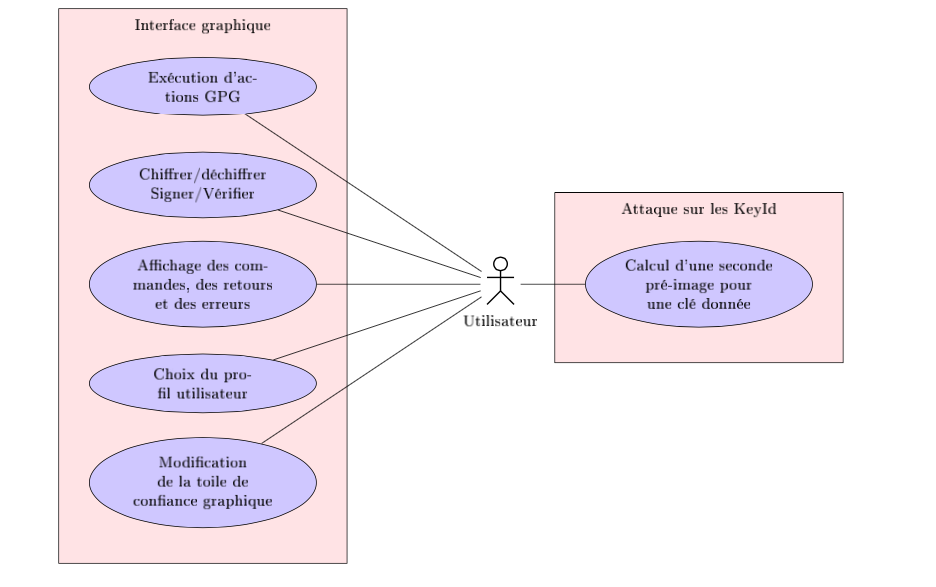
\includegraphics[scale=0.4]{usecase.png}
  
  \medbreak
  
  L'attaque sur les KeyId est indépendante et ne fera pas partie de l'interface graphique. 
  
  \subsection{Contraintes}
  
  L'application doit fonctionner sur le système d'exploitation GNU/Linux, en particulier sous les environnements KDE et Gnome.
  L'interface doit être à la fois pédagogique et précise pour faciliter l'utilisation de GPG. 
  
  \subsection{Organisation}

\section{Présentation du projet final}
  \subsection{Objectifs}
    Pendant le développement du projet, deux membres nous ont quittés (Bertille et Guillaume), ce qui nous a forcé à revoir toute notre planification, n'ayant plus les moyens humains pour tenir le rythme prévu.
  \subsection{Organisation}
    
    Le projet a été replanifié et découpé en deux livraisons.
    L'attribution des tâches a été refaite, avec la répartition suivante :
    \begin{itemize}
      \item Ibrahima sur l'étude de GPG,
      \item Lucas sur l'attaque sur les KeyID,
      \item Les autres (Matthieu, Olivier et Pierre) sur le développement de l'application.
    \end{itemize}

  \subsection{Fonctionnalités}
    Les fonctionnalités ayant été complétées sont :\medbreak
  \begin{itemize}
  \item Exécution d'actions GPG \smallbreak
  Création, exportation, importations de clés (en local)\smallbreak
  \item Chiffrer / déchiffrer / signer / vérifier \smallbreak
  Chiffrer ou déchiffrer ou signer ou vérifier un fichier. \smallbreak
  \item Affichage des commandes, des retours et des erreurs \smallbreak
  L'utilisateur peut choisir d'afficher ou non les commandes, les retours et les erreurs associés à chaque action GPG. \smallbreak 
  \item Création / Modification / Suppression du profil utilisateur \smallbreak
  \item Modification de la toile de confiance \smallbreak
  Modification de la toile de confiance par un changement de niveau de confiance, l'ajout d'une nouvelle clé ou la modification d'une clé. \smallbreak
  \item Calcul d'une seconde pré-image pour une clé donnée \smallbreak
  Attaque permettant d'obtenir une nouvelle clé contenant le même KeyId que la première.
  \end{itemize}


  

  Les fonctionnalités qui ont été supprimées par rapport au plan initial sont :\medbreak
  \begin{itemize}
  \item Toile de confiance graphique\smallbreak
  Représentation de la toile de confiance sous forme de graphe\smallbreak
  \item Chiffrer / déchiffrer / signer / vérifier \smallbreak
  Chiffrer ou déchiffrer ou signer ou vérifier le texte contenu dans l'éditeur de l'interface.\smallbreak
  \item Edition de clé \smallbreak
  Quelques fonctions d'édition de clé ne sont pas implémentées, comme la révocation d'une clé ou la signature avec une clé en particulier \smallbreak 
  

  La partie interface graphique a été validée par le client, mais malheureusement l'attaque et l'étude sur GPG n'ont pas été validés car ils n'ont pas été rendus à temps.

  \end{itemize}

\section{Les problèmes rencontrés}

  \subsection{Problèmes organisationnel}
    \subsubsection{Équipe}
    \subsubsection{Planning}
    
  \subsection{Problèmes techniques}
    \subsubsection{Maîtrise des outils}
    \subsubsection{Maîtrise de GnuPG}
    \subsubsection{Communication GnuPG}
  

\section{Bilan du projet}
  \subsection{Compétences acquises}
    \subsubsection{Technique}
    \subsubsection{Organisationnel}
  \subsection{Axes d'amélioration}
  \subsection{Rétrospective}

\section{Conclusion}



\end{document}

